\begin{frame}{Allgemeines}{Wer bin ich?}
		\begin{itemize}
			\item Lukas Abelt
			\item <2-> 21 Jahre (Jahrgang '97)
			\item <3-> Ursprünglich aus Werder (Havel)
			\begin{itemize}
				\item <4->...in Brandenburg
				\item <5->...bei Potsdam
				\begin{itemize}
					\item <6->...bei Berlin
				\end{itemize}
			\end{itemize}
		\end{itemize}
	\end{frame}
	
	\begin{frame}{Allgemeines}{Wo komme ich her?}
		\begin{figure}
		\centering
			\begin{minipage}{0.7\textwidth}
			\centering
			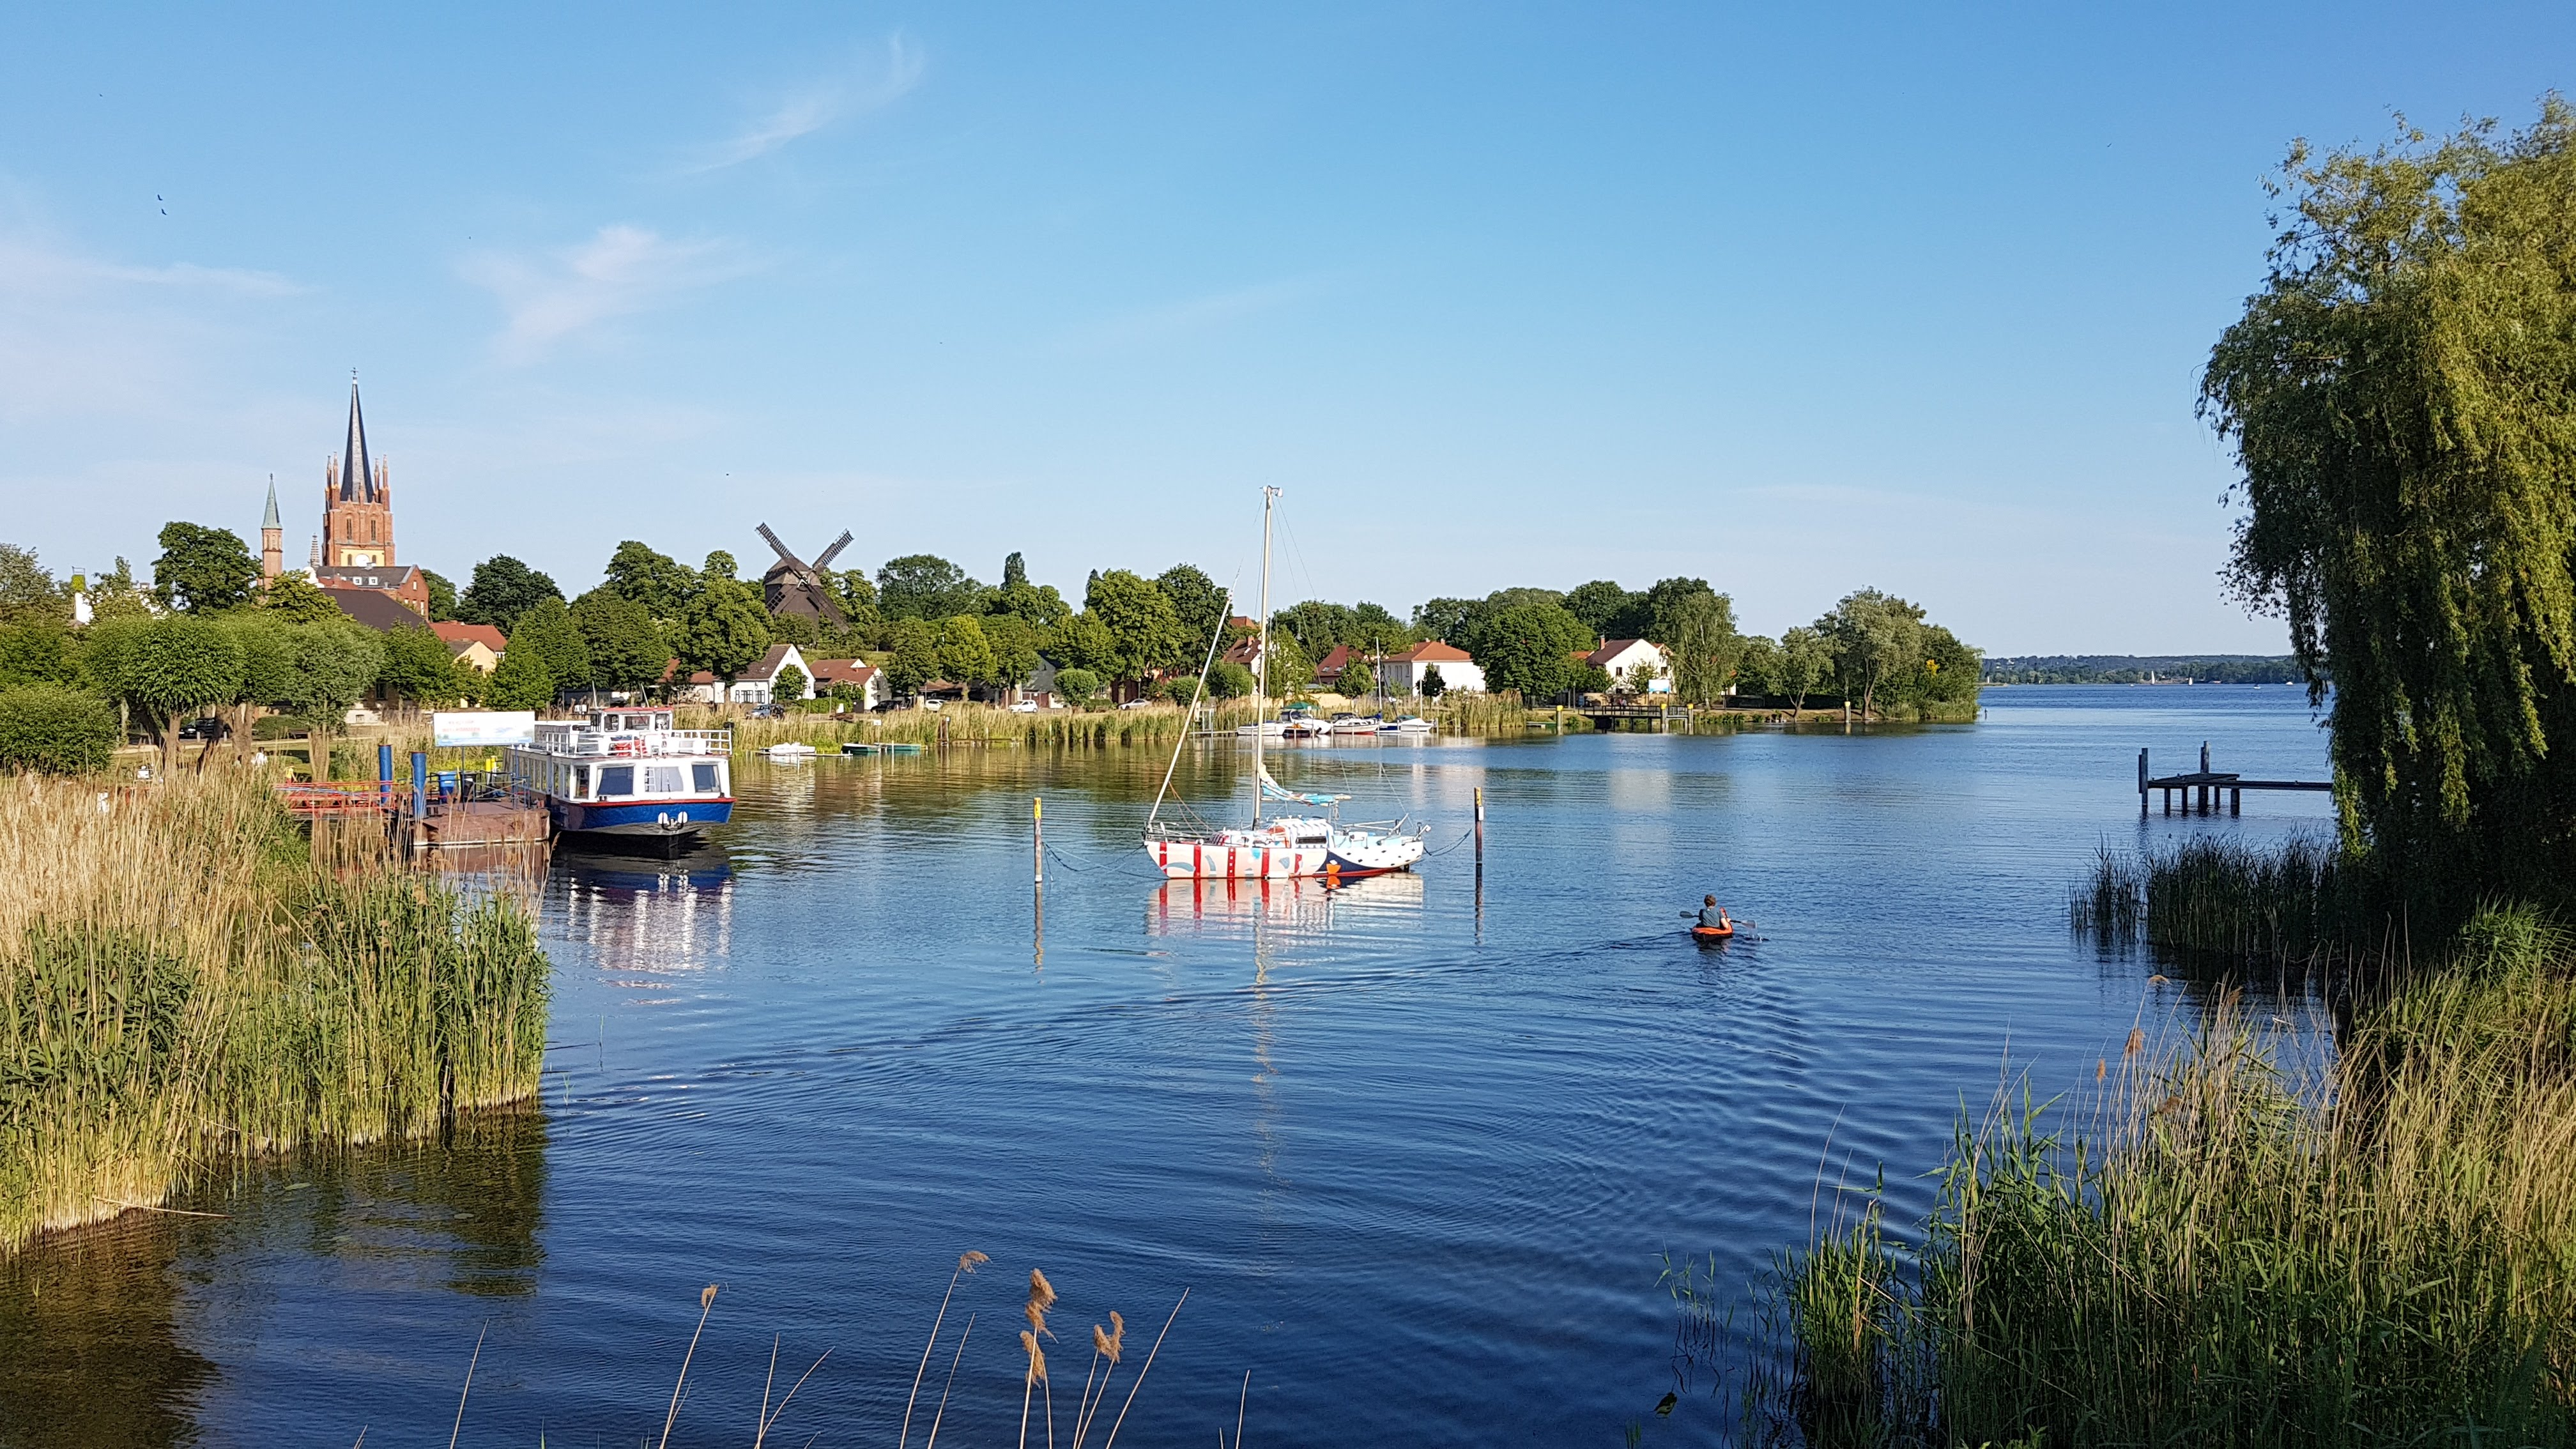
\includegraphics[width=.95\linewidth]{graph/werder.jpg}
			\end{minipage}%
			\begin{minipage}{0.3\textwidth}
			\centering
			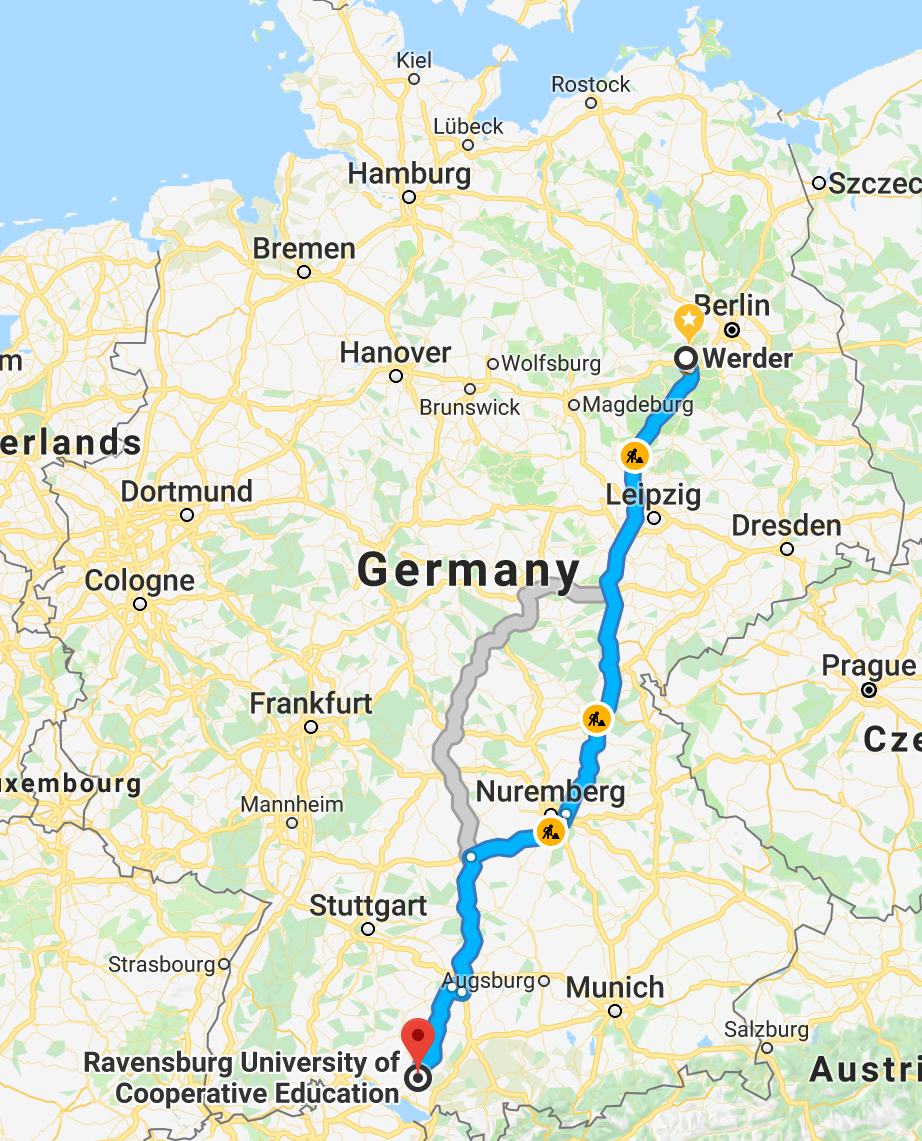
\includegraphics[width=.95\linewidth]{graph/route2werder.png}
			\end{minipage}
		\end{figure}
	\end{frame}

	\begin{frame}{Beruflicher\&Akademischer Werdegang}{}
		\begin{itemize}
			\item \textbf{Juli 2015} - Abitur
			\item \textbf{Ab September 2015} - Duales Studium
			\begin{itemize}
				\item Hochschule: DHBW Ravensburg \textbf{Campus Friedrichshafen}
				\item Studiengang: Informationstechnik (Mobile Informatik)
				\item Firma: Airbus Defence and Space (Immenstaad)
			\end{itemize}
			\item \textbf{September 2018} - Bachelorarbeit und -abschluss
			\item \textbf{Seit Oktober 2018} - Software Architect bei Airbus
		\end{itemize}
	\end{frame}
	
	\begin{frame}{Was habe ich bisher gemacht?}{Praxisphasen}
			\begin{itemize}
				\item Arbeit im Bereich SIGINT(Signal Intelligence)
				\item Implementierung des TCP Stacks zur Übertragung von Signaldaten(C++, Matlab, Simulink)
				\item Später Abteilungswechsel zu Simulationssoftware
				\item Implementierung eines neuen Schadenmodells in das bestehende System (C++)
				\item \textbf{Analyse und Bewertung neuer Methoden zur Durchführung simulationsgestützter Parameterstudien mit cloud-basierten Systemen} (Bachelorarbeitsthema)
			\end{itemize}
	\end{frame}
	
	\begin{frame}{Was habe ich bisher gemacht?}{Theoriephasen}
		\begin{itemize}
			\item Mathetutorium für Semester 1
			\item Mathetutorium für Semester 2
			\item Studienarbeit: Entwickeln eines selbstlernenden Chatbots (Tensorflow, Python)
			\begin{itemize}
				\item Erfolgreiche Zielerreichung fraglich?
			\end{itemize}
			\item 3. Platz beim Bierathlon 2016
			\item Organisator des alljährlichen Glühweingrillens Friedrichshafen (Nächster Termin: April 2019)
		\end{itemize}
	\end{frame}
	
	\begin{frame}{Was habe ich bisher gemacht?}{Studienarbeit}
		"they're just fucking fucking fucking not just fucking with"
	\end{frame}